\section{Assignment 7}

\subsection{Implement the Tank-based bilateral teleoperation architecture for the F-P and P-P cases}

\begin{figure}[h]
\centering
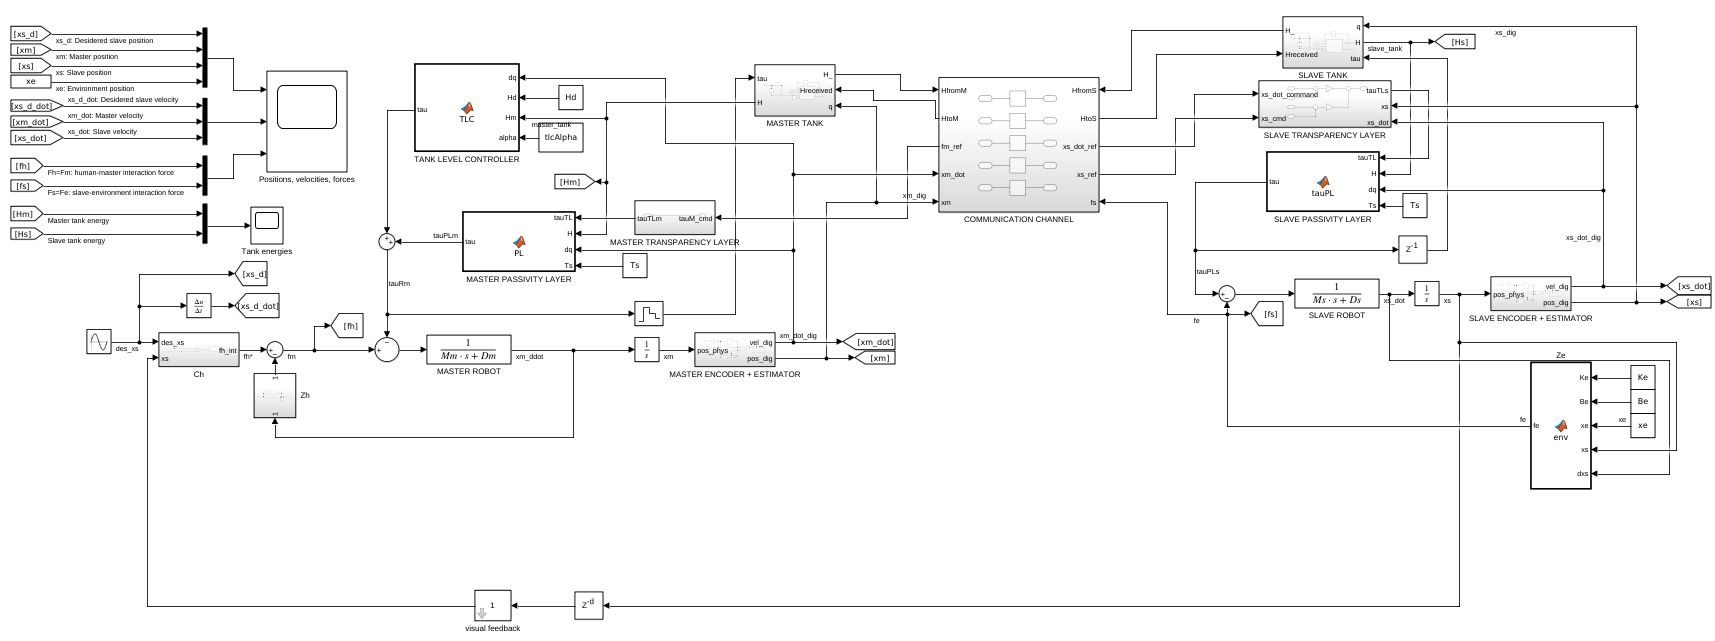
\includegraphics[keepaspectratio,width=\textwidth]{tank_fp}
\caption{Tank-based F-P teleoperation architecture}
\end{figure}

\begin{figure}[h]
\centering
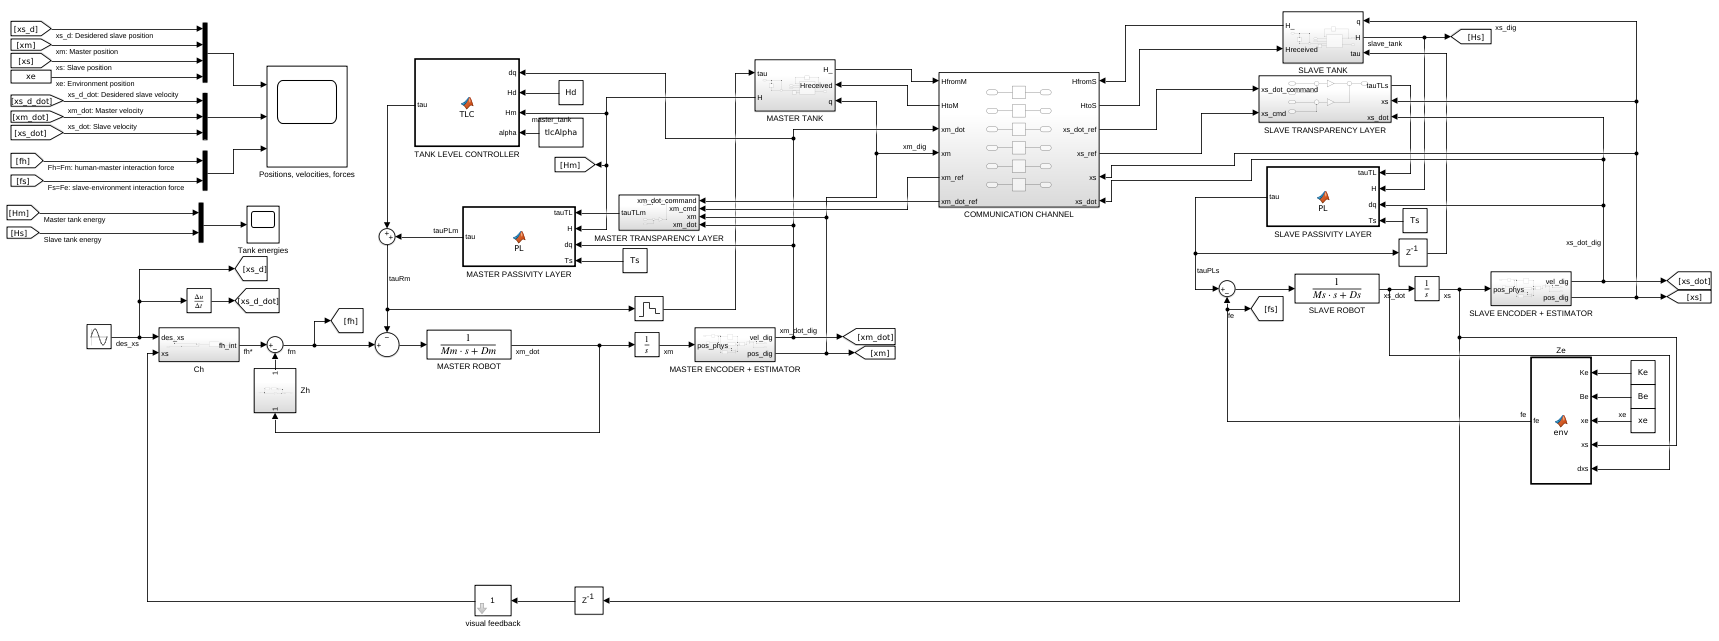
\includegraphics[keepaspectratio,width=\textwidth]{tank_pp}
\caption{Tank-based P-P teleoperation architecture}
\end{figure}

The tank-based teleoperation architecture uses a two-layer control architecture that combines passivity (and therefore stability) and transparency (and therefore high teleoperation performance). The layers, in hierarchical order, are:

\begin{itemize}
\item Passivity layer: introduces passivity, and therefore stability, into the system by absorbing the energy generated by communication delays or environment interaction forces.
\item Transparency layer: implements the control structure that ensures transparency of the teleoperation system, taking into account information about the system, environment and task the user is executing.
\end{itemize}

Both layers contribute some energy to an energy tank. The level of the tank represents the energy budget available to be used to carry out robot motions. The energy in the tank can only be replenished by the user at the master side.

To separate the passivity and transparency layers, a tank level controller (TLC) is introduced in the passivity layer at the master side. The role of the TLC is to regulate the tank's energy content,  ensuring it remains in a stable range. 

\subsection{Compare positions, velocities, forces, commands in free motion and in contact}

\begin{figure}[H]
\begin{minipage}{0.5\textwidth}
\centering
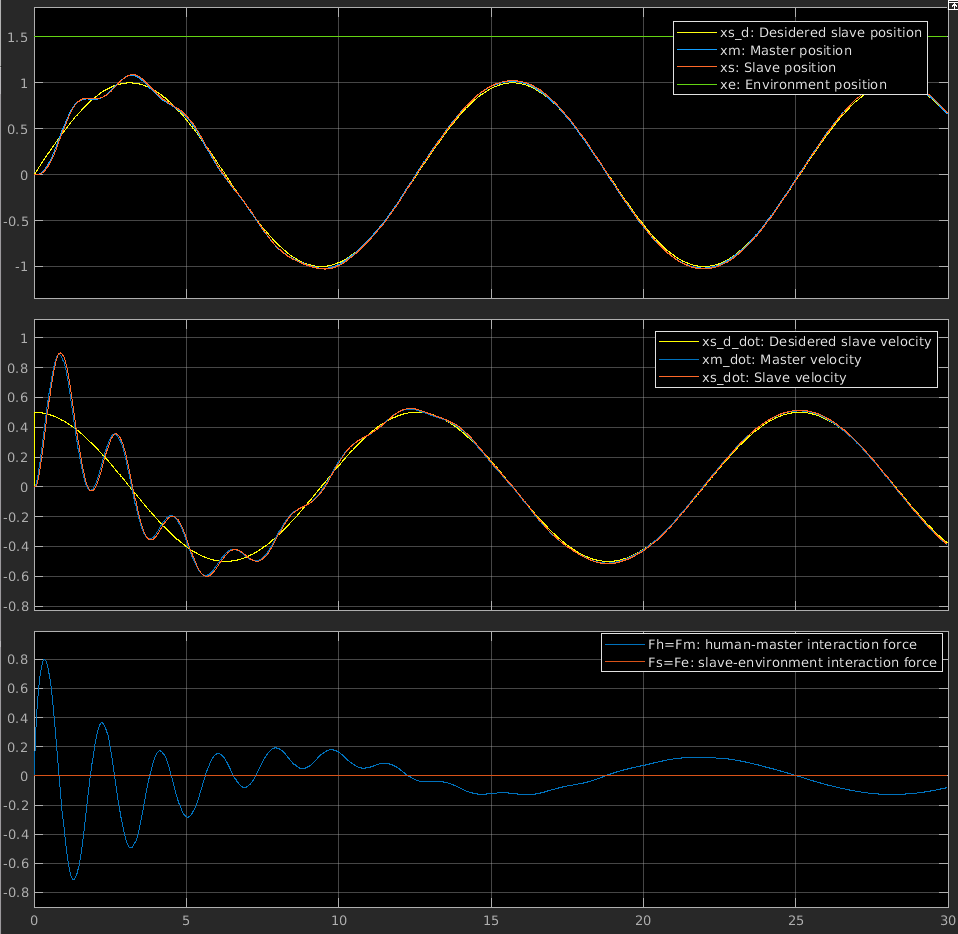
\includegraphics[keepaspectratio,width=\textwidth]{tfp_free_nok}
\caption{FP in free motion, without noise}
\label{fig:tfp_free_nok}

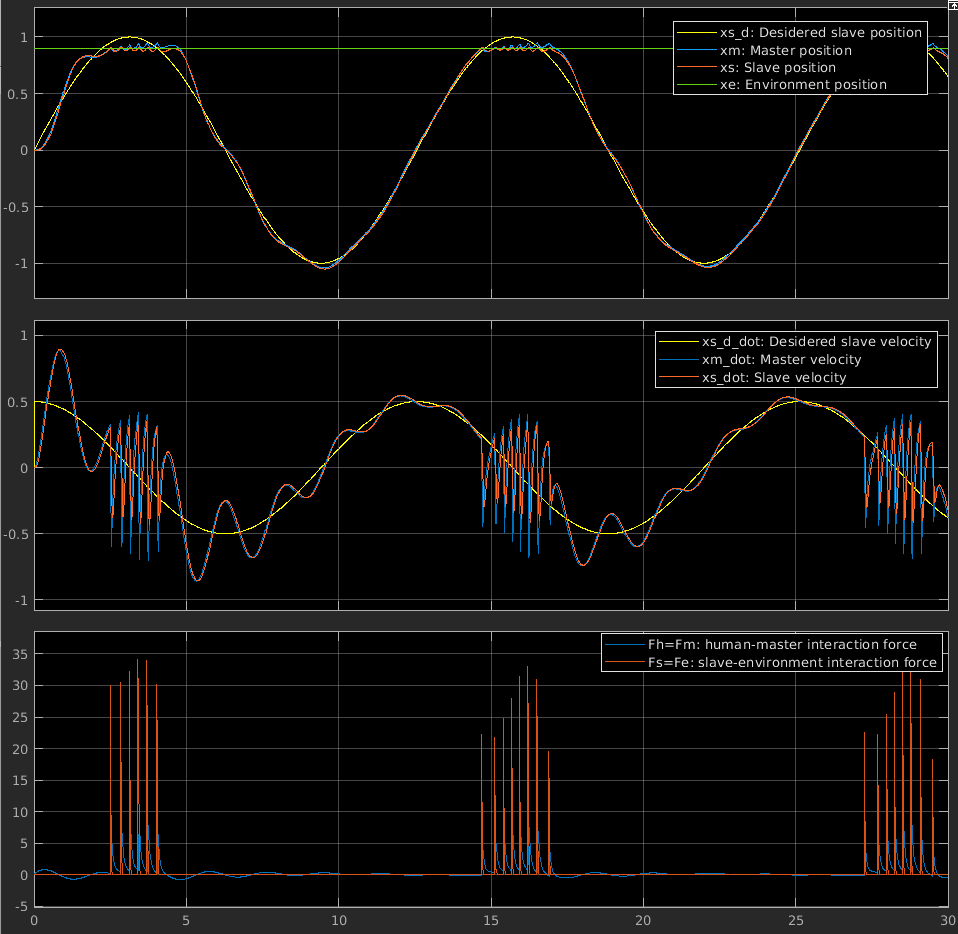
\includegraphics[keepaspectratio,width=\textwidth]{tfp_contact_nok}
\caption{FP in contact, without noise}
\label{fig:tfp_contact_k}
\end{minipage}
\begin{minipage}{0.5\textwidth}
\centering
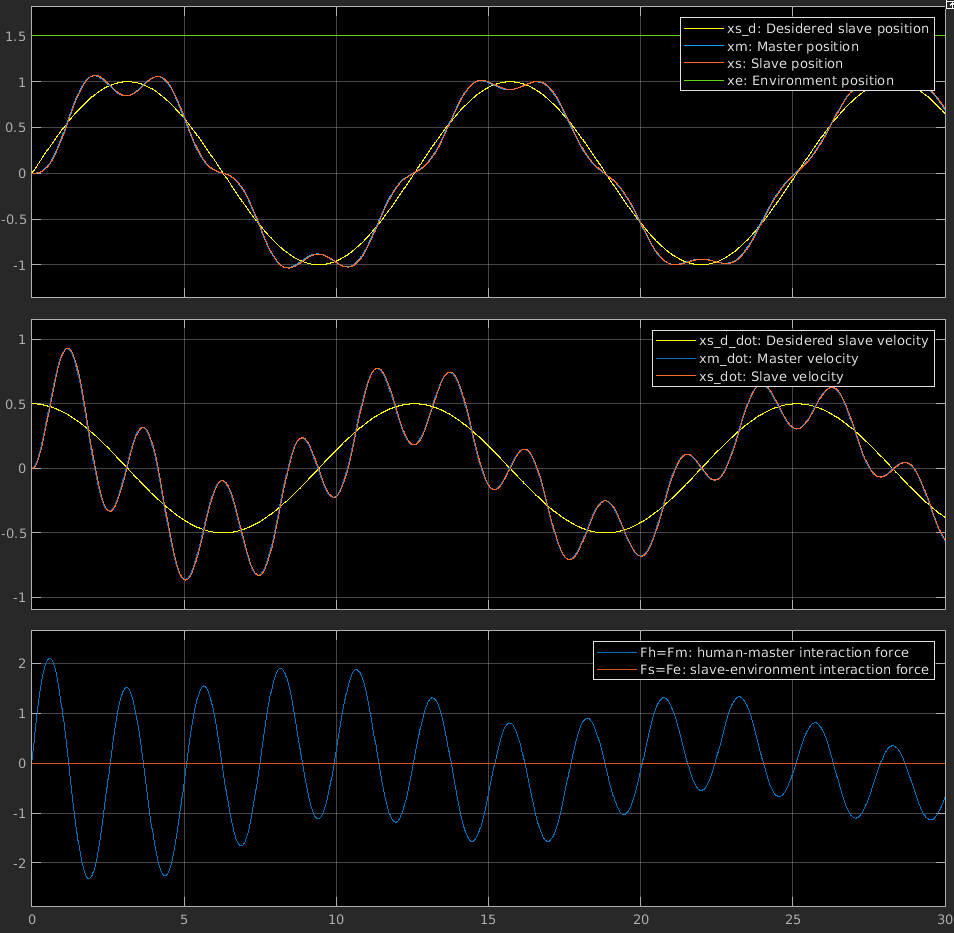
\includegraphics[keepaspectratio,width=\textwidth]{tpp_free_nok}
\caption{PP in free motion, without noise}
\label{fig:tpp_free_nok}

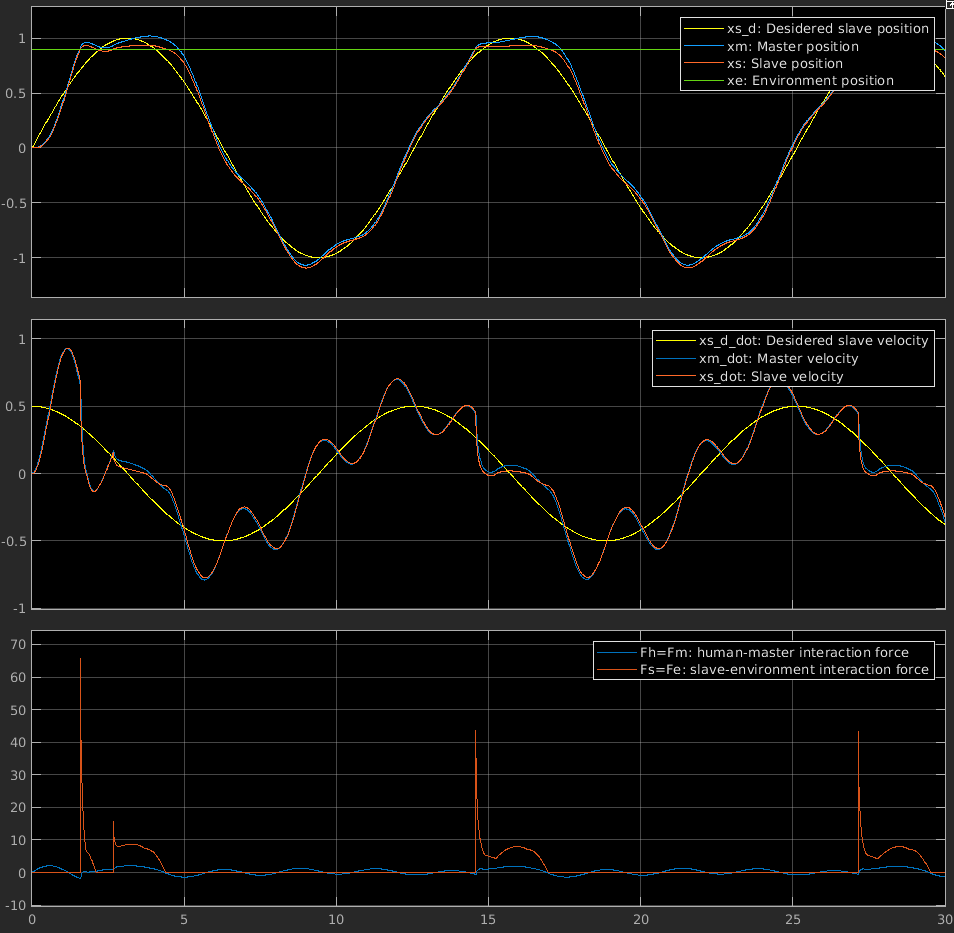
\includegraphics[keepaspectratio,width=\textwidth]{tpp_contact_nok}
\caption{PP in contact, without noise}
\label{fig:tpp_contact_nok}
\end{minipage}
\end{figure}

\subsection{Create another simulink model and (a) add the measurement noise to the position/force signals, and (b) estimate velocities from positions}

\begin{figure}[H]
\begin{minipage}{0.5\textwidth}
\centering
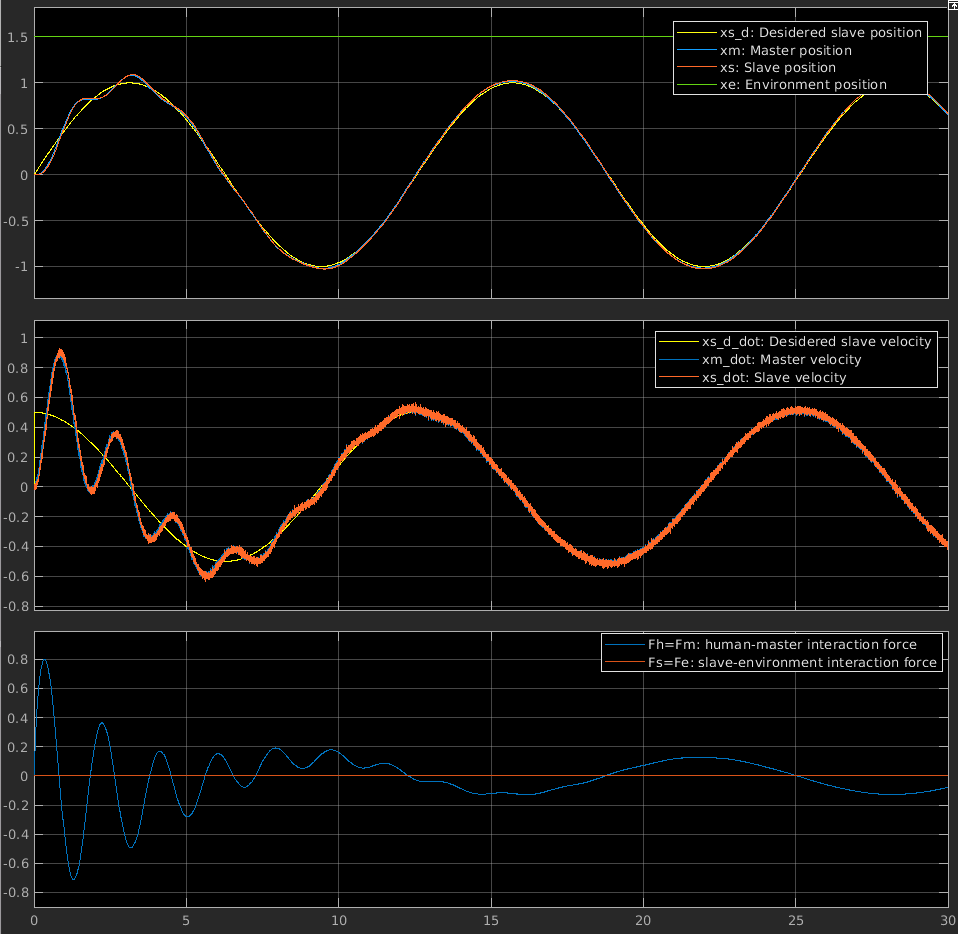
\includegraphics[keepaspectratio,width=\textwidth]{tfp_free_k}
\caption{FP in free motion, with noise}
\label{fig:spp_free_nok}

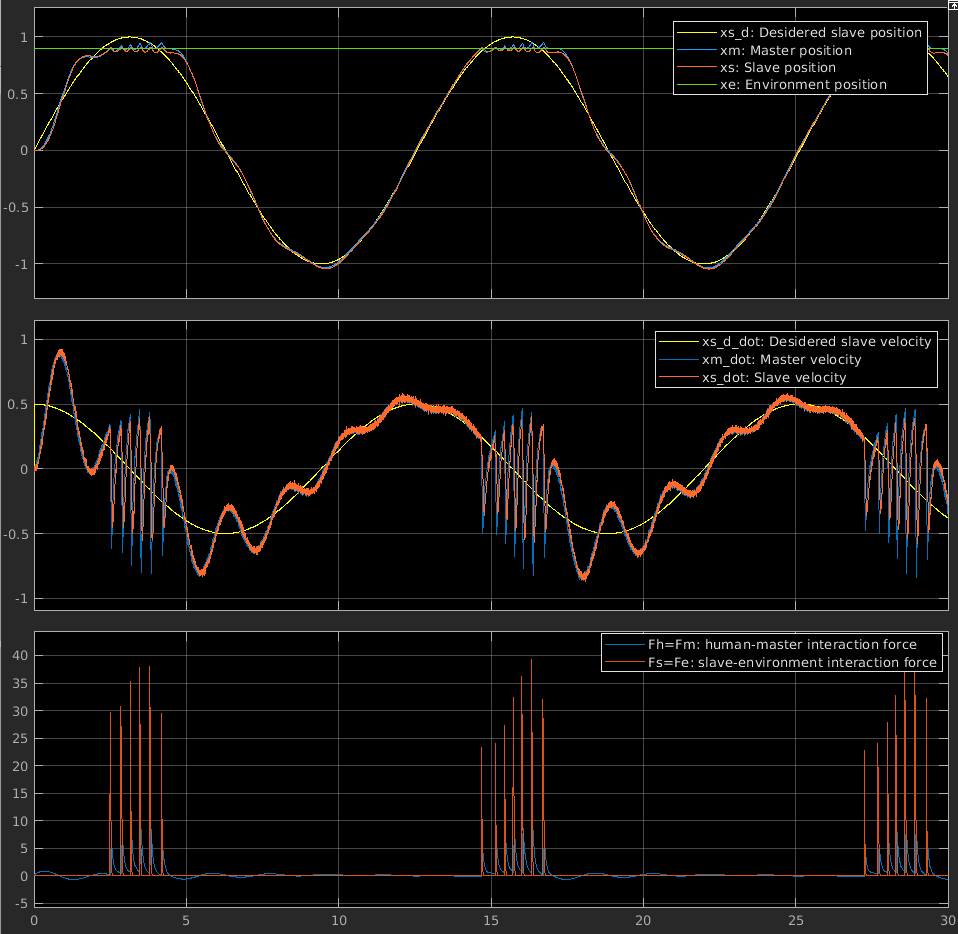
\includegraphics[keepaspectratio,width=\textwidth]{tfp_contact_k}
\caption{FP in contact, with noise}
\label{fig:spp_free_k}
\end{minipage}
\begin{minipage}{0.5\textwidth}
\centering
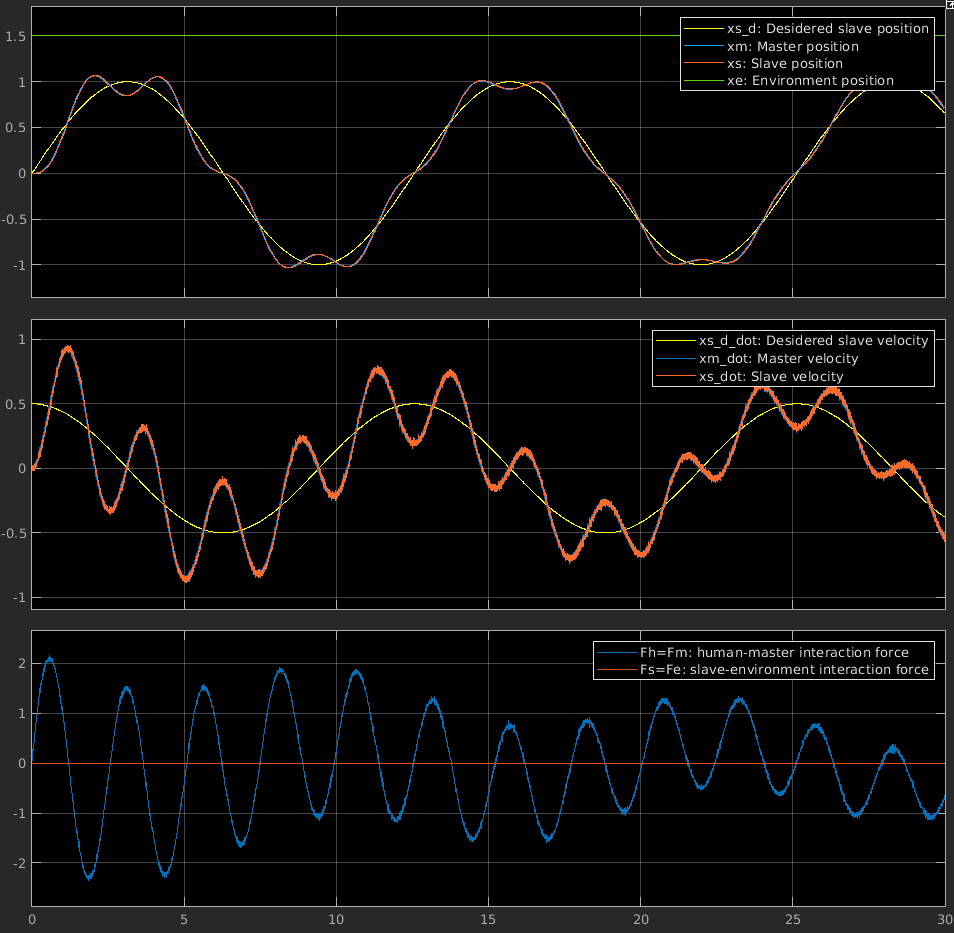
\includegraphics[keepaspectratio,width=\textwidth]{tpp_free_k}
\caption{PP in free motion, with noise}
\label{fig:spp_contact_nok}

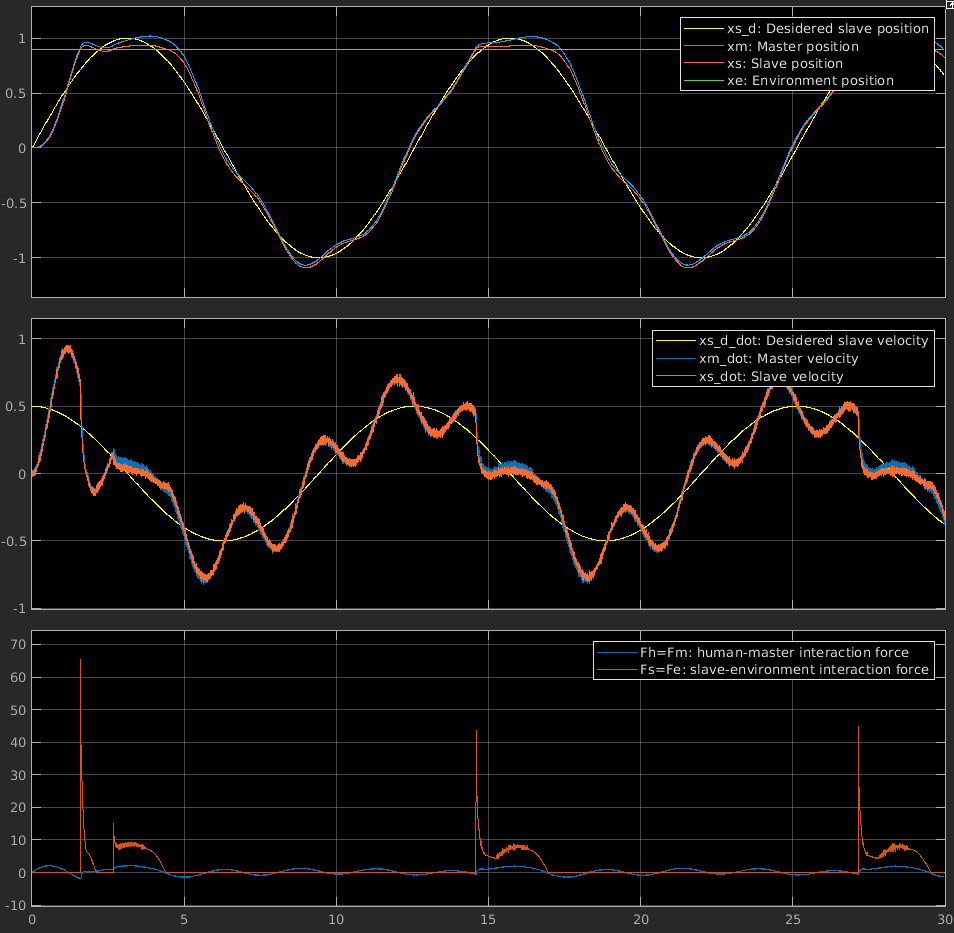
\includegraphics[keepaspectratio,width=\textwidth]{tpp_contact_k}
\caption{PP in contact, with noise}
\label{fig:spp_contact_k}
\end{minipage}
\end{figure}

\subsection{PP - Tank energy levels}

\begin{figure}[H]
\begin{minipage}{0.5\textwidth}
\centering
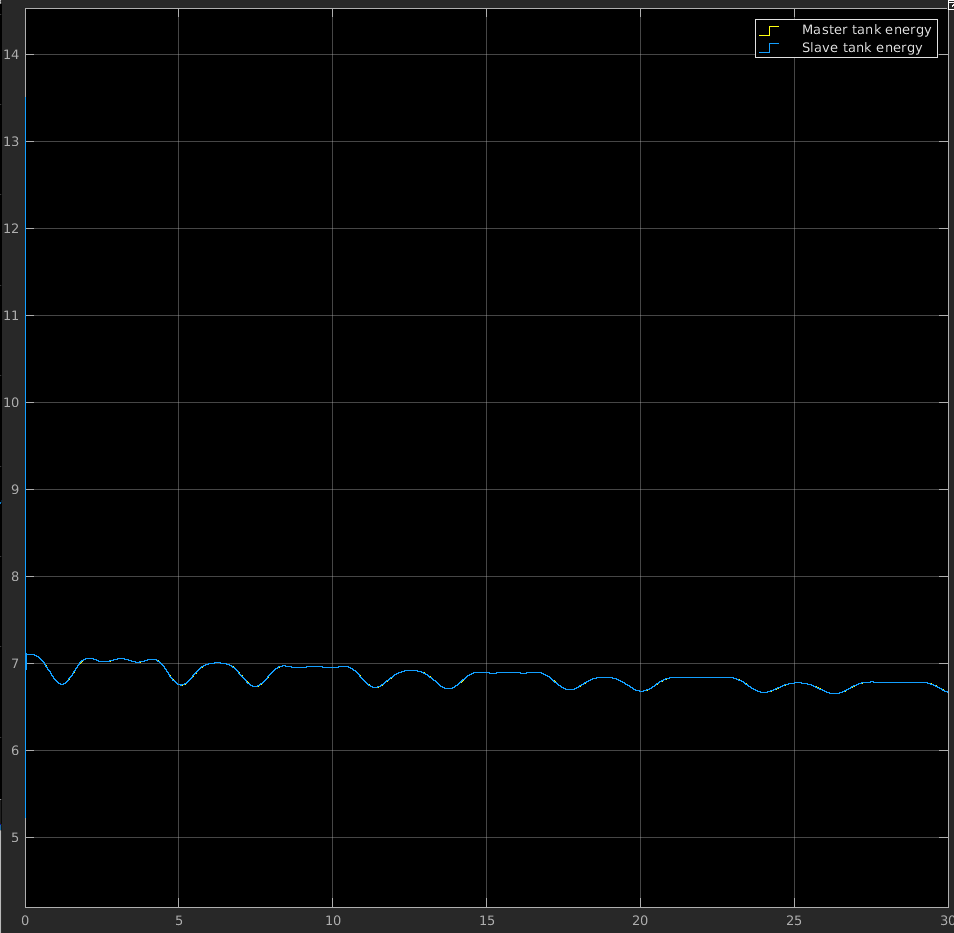
\includegraphics[keepaspectratio,width=\textwidth]{tpp_free_energy}
\caption{Free motion, initial tank energy $H_m=H_s=15$}
\medskip
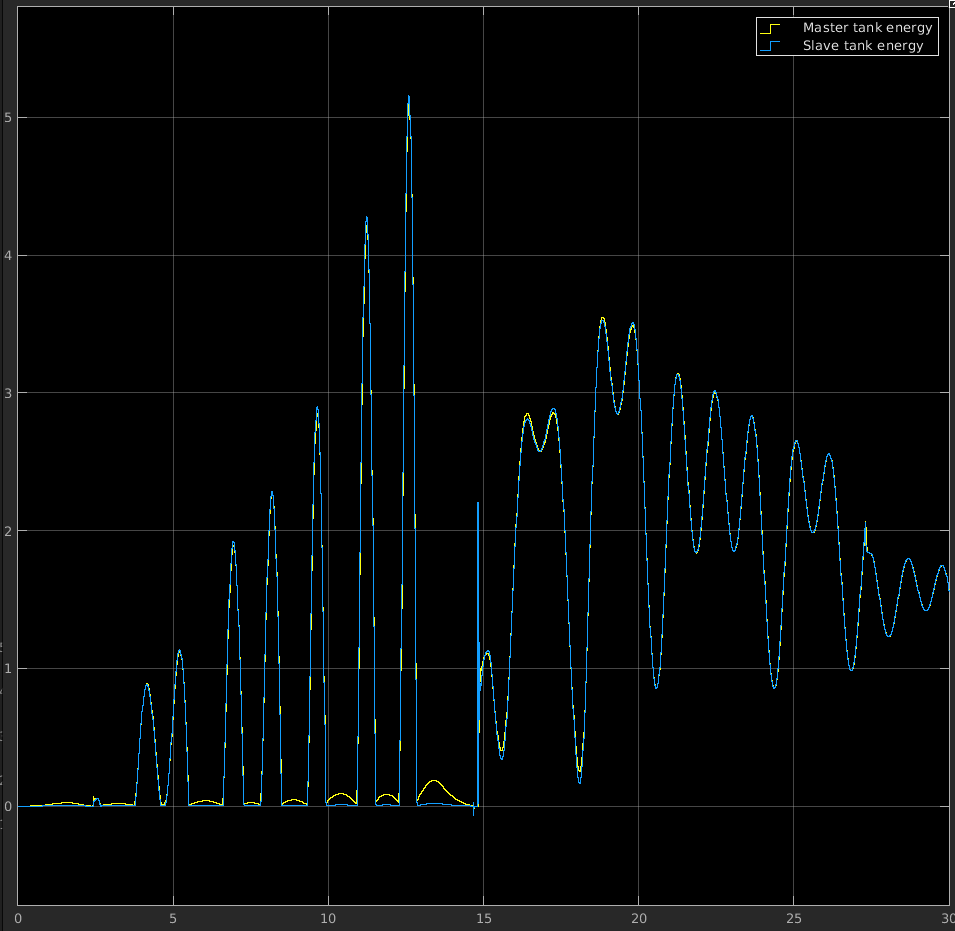
\includegraphics[keepaspectratio,width=\textwidth]{tpp_free_0energy}
\caption{Free motion, initial tank energy $H_m=H_s=0$}
\end{minipage}
\begin{minipage}{0.5\textwidth}
\centering
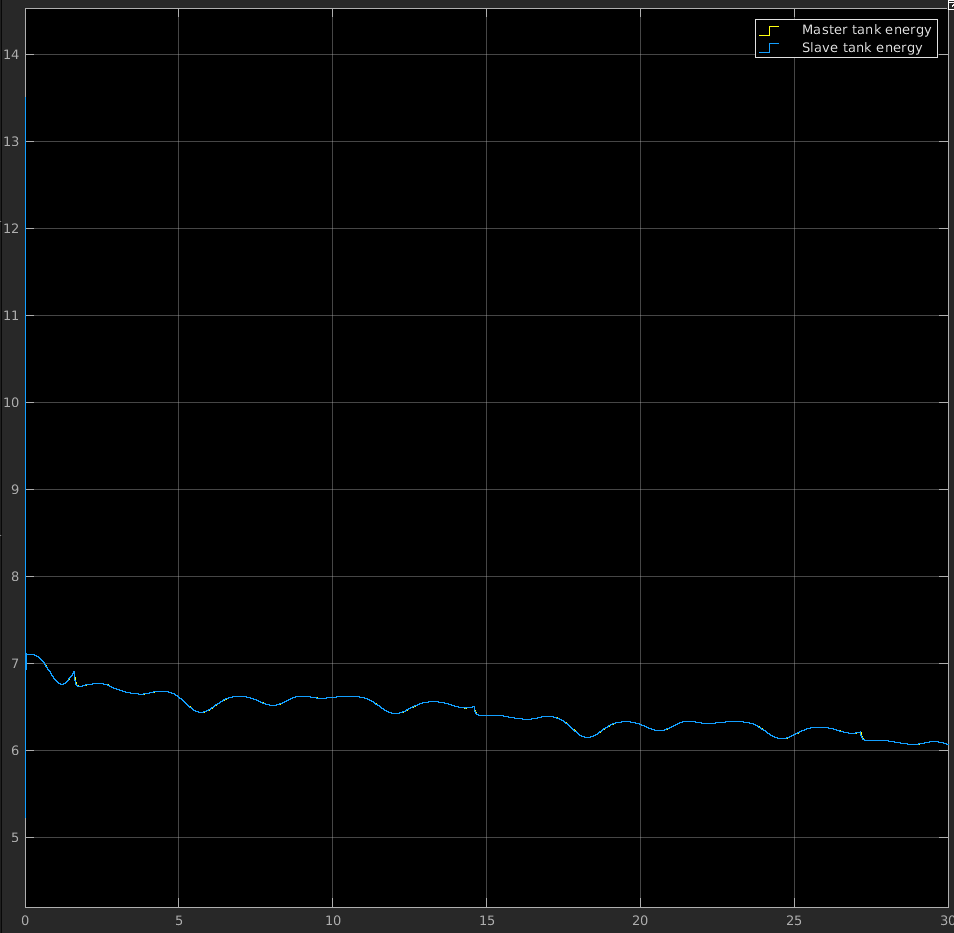
\includegraphics[keepaspectratio,width=\textwidth]{tpp_contact_energy}
\caption{Contact, initial tank energy $H_m=H_s=15$}
\medskip
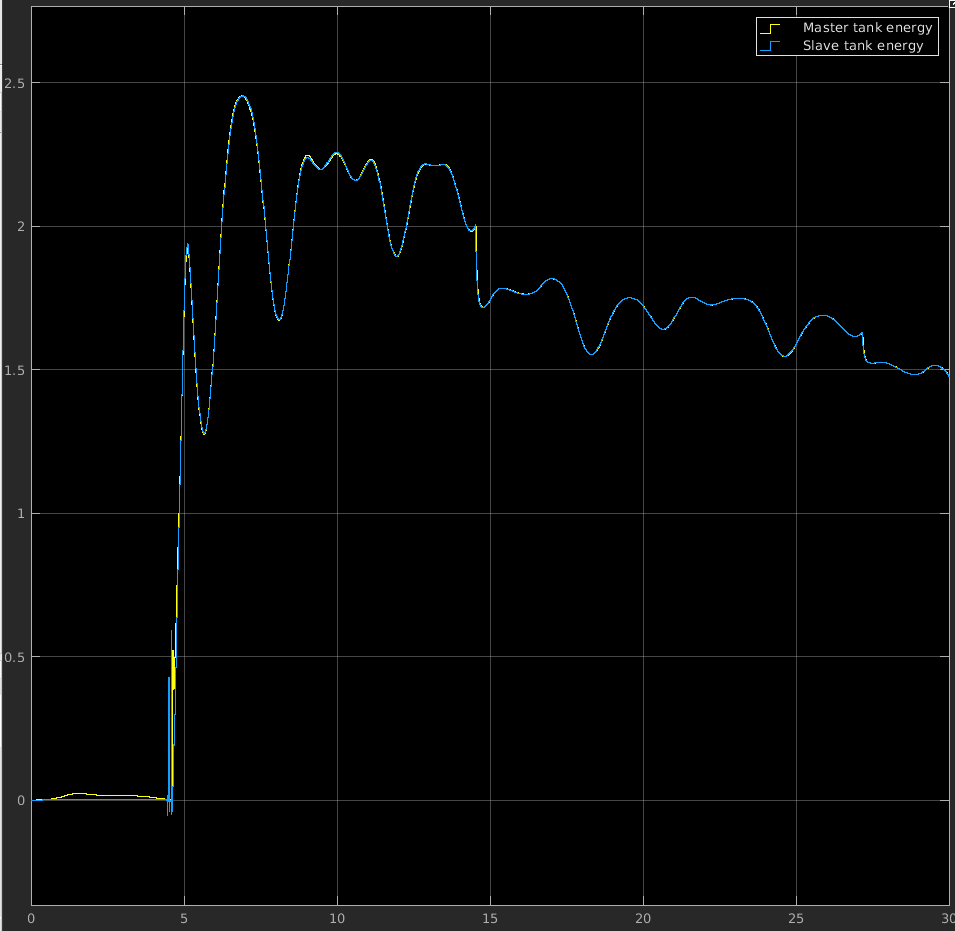
\includegraphics[keepaspectratio,width=\textwidth]{tpp_contact_0energy}
\caption{Contact, initial tank energy $H_m=H_s=0$}
\end{minipage}
\end{figure}

\begin{figure}
\centering
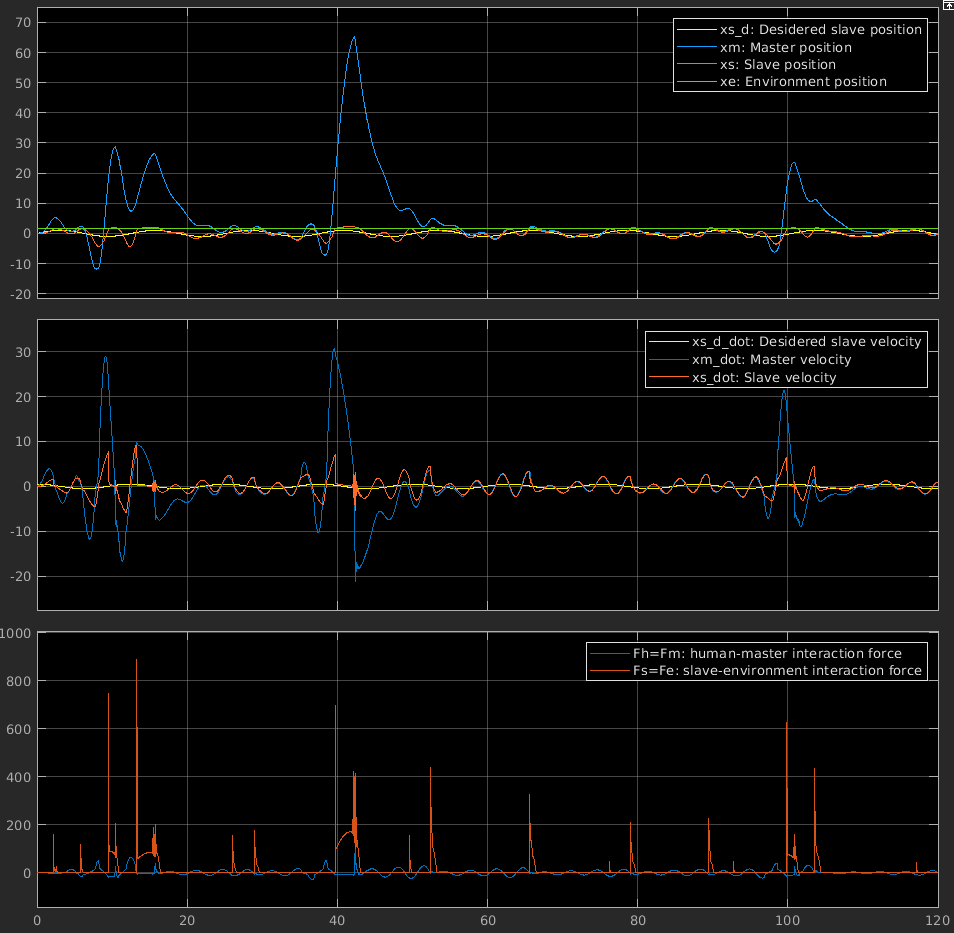
\includegraphics[keepaspectratio,width=\textwidth]{tank_pp_longsim}
\caption{Free motion, initial tank energy $H_m=H_s=0$, longer simulation time}
\end{figure}

\begin{figure}
\centering
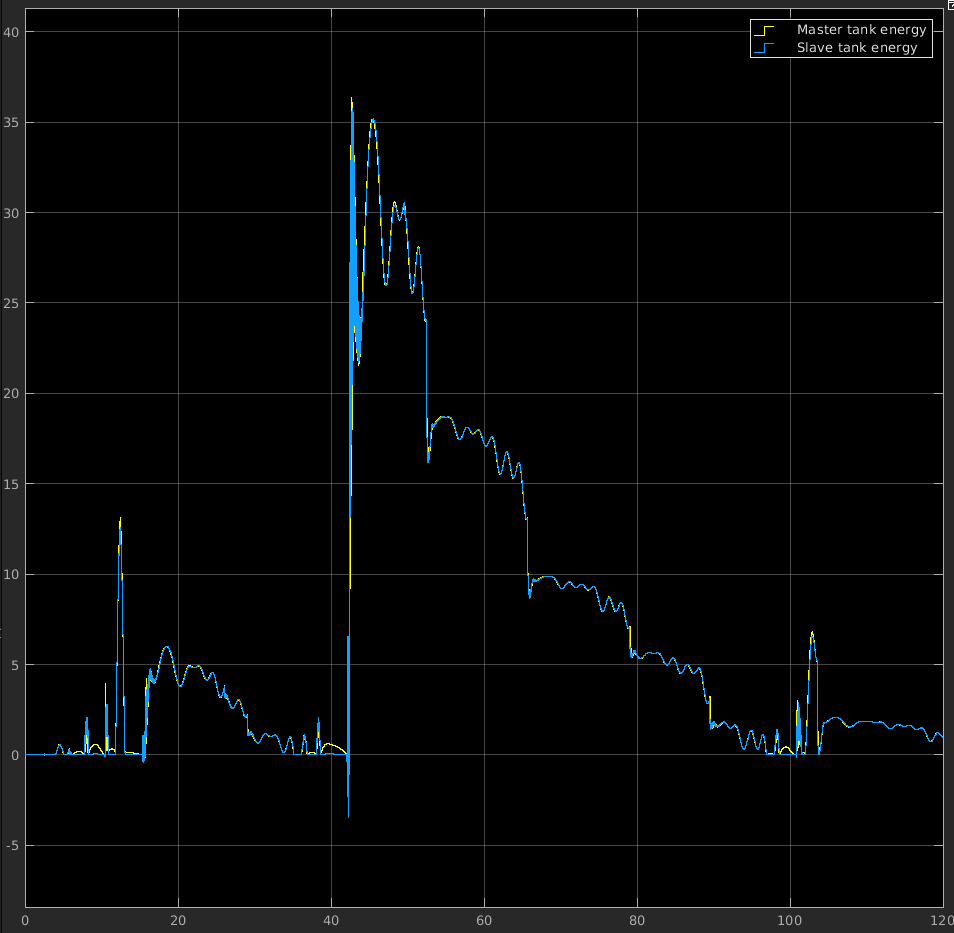
\includegraphics[keepaspectratio,width=\textwidth]{tank_pp_longsim_energy}
\caption{Free motion, initial tank energy $H_m=H_s=0$, longer simulation time}
\end{figure}

\newpage

\subsection{FP - Tank energy levels}

\begin{figure}[H]
\begin{minipage}{0.5\textwidth}
\centering
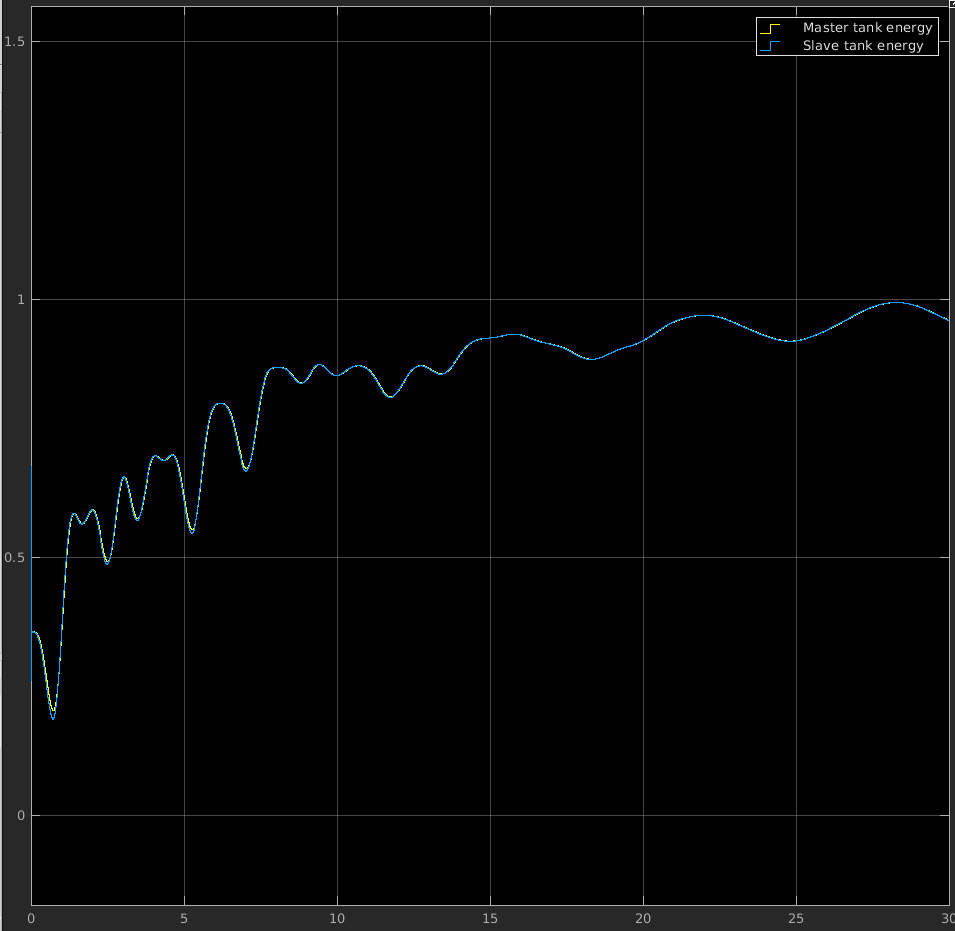
\includegraphics[keepaspectratio,width=\textwidth]{tfp_energy}
\caption{Free motion, initial tank energy $H_m=H_s=0.5$}
\end{minipage}
\begin{minipage}{0.5\textwidth}
\centering
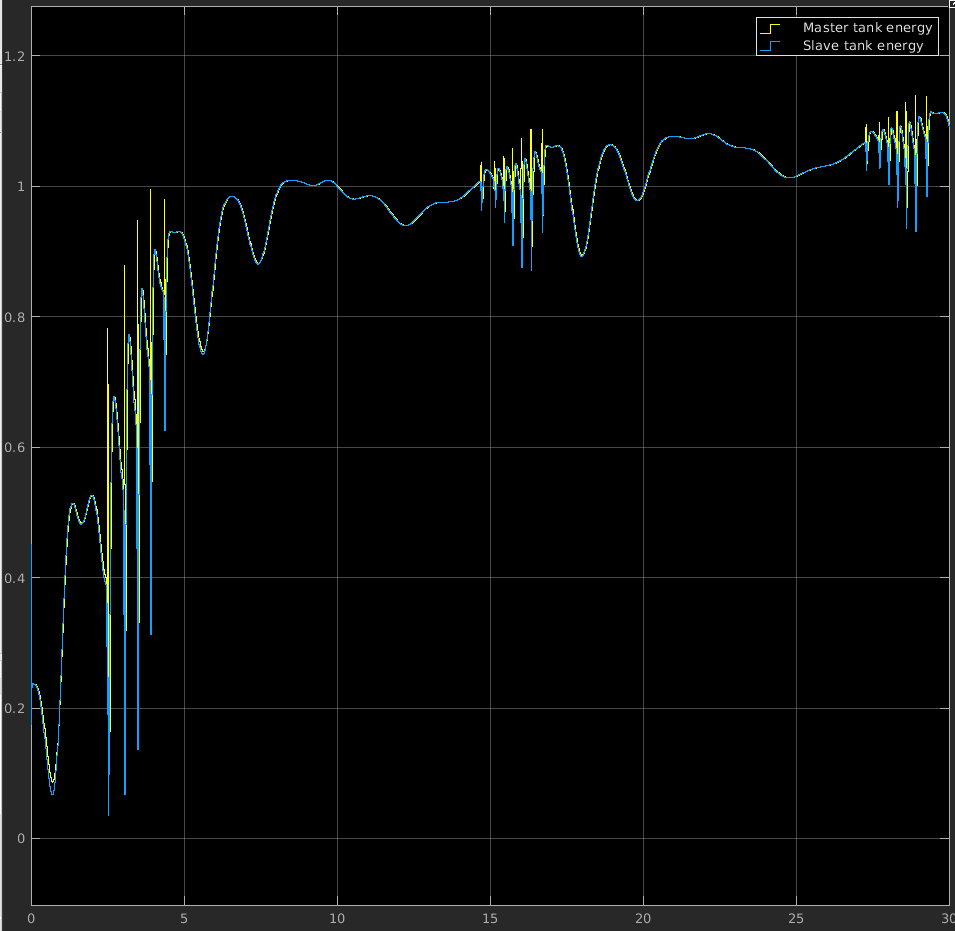
\includegraphics[keepaspectratio,width=\textwidth]{tfp_energy_contact}
\caption{Contact, initial tank energy $H_m=H_s=0.5$}
\end{minipage}
\end{figure}